% !TeX root = enterprise-architecture-digital-blueprint.tex
% !TeX encoding = UTF-8
\chapter{Arsitektur Data dan Informasi Saat Ini}

\section*{Tujuan Pembelajaran}
\begin{itemize}
  \item Mengidentifikasi konsep informasi bisnis utama beserta pemiliknya.
  \item Memetakan lokasi dan aliran data penting di antara aplikasi dengan matriks
        CRUD (\textit{Create, Read, Update, Delete}).
  \item Menganalisis masalah kualitas, duplikasi, dan klasifikasi data yang
        menghambat strategi.
\end{itemize}

\section{Pendahuluan}

Rapat direksi Medikara Health pada November 2025 berhenti di satu angka.
Direktur Keuangan melaporkan 99.870 kunjungan pasien sepanjang Oktober,
sedangkan Direktur Pelayanan membawa angka 102.640. Selisihnya 2.770
kunjungan, dan tidak ada yang salah menghitung. Angka pertama diambil langsung
dari lima SIMRS (Sistem Informasi Manajemen Rumah Sakit). Angka kedua berasal
dari rekap \textit{spreadsheet} yang menggabungkan ekspor tujuh aplikasi, termasuk
telekonsultasi di Medikara+. Kedua angka memakai arti "kunjungan" yang
berbeda, dan rapat menghabiskan setengah jam hanya untuk menyepakati angka
mana yang dipakai.

Kejadian seperti itu adalah gejala, bukan penyakitnya. Penyakitnya ada pada
arsitektur data: data pasien tersebar di lima SIMRS dengan versi berbeda,
aplikasi Medikara+ milik vendor, ERP (\textit{Enterprise Resource Planning})
keuangan, dan puluhan berkas \textit{spreadsheet}. Tidak ada yang tahu pasti di
mana satu data dibuat, siapa yang berhak mengubahnya, dan seberapa sensitif
isinya. Bab 5 memotret apa yang mampu dilakukan Medikara lewat
\textit{capability map}. Bab ini memotret bahan baku yang dipakai kapabilitas
itu, yaitu data. Dalam ADM (\textit{Architecture Development Method}), pekerjaan
ini termasuk fase C untuk domain data pada kondisi saat ini (\textit{baseline}).
Hasilnya tiga artefak untuk tonggak C2: peta informasi, matriks CRUD, dan
daftar masalah data. Bab 9 memakai ketiganya untuk merancang identitas pasien
tunggal.

Rujukan utama bab ini terbagi tiga. Dari sisi arsitektur, TOGAF
(\textit{The Open Group Architecture Framework}) menyediakan katalog, matriks,
dan diagram untuk domain data \cite{togaf10}, BIZBOK (\textit{Business
Architecture Body of Knowledge}) menyediakan cara menyusun peta informasi
\cite{bizbok15}, dan ArchiMate 3.2 menyediakan elemen untuk memodelkannya
\cite{archimate32}. Dari sisi pengelolaan data, DAMA-DMBOK (\textit{Data
Management Association, Data Management Body of Knowledge}) menjadi acuan
untuk data induk dan kualitas data \cite{dmbok2}, dilengkapi kajian Wang
dan Strong tentang arti kualitas data bagi pemakainya \cite{c06-wang1996}.
Dari sisi regulasi, bab ini memakai Undang-Undang (UU) Nomor 27 Tahun 2022
tentang Pelindungan Data Pribadi \cite{uu27-2022-pdp} dan Peraturan Menteri
Kesehatan (Permenkes) Nomor 24 Tahun 2022 tentang Rekam Medis
\cite{permenkes24-2022}.

\IfFileExists{../figures/ch06-diagram-konsep.png}{%

Gambar \ref{fig:ch06-ilustrasi-bab} merangkum hubungan komponen dan konsep utama bab ini.
\begin{figure}[!htb]
  \centering
  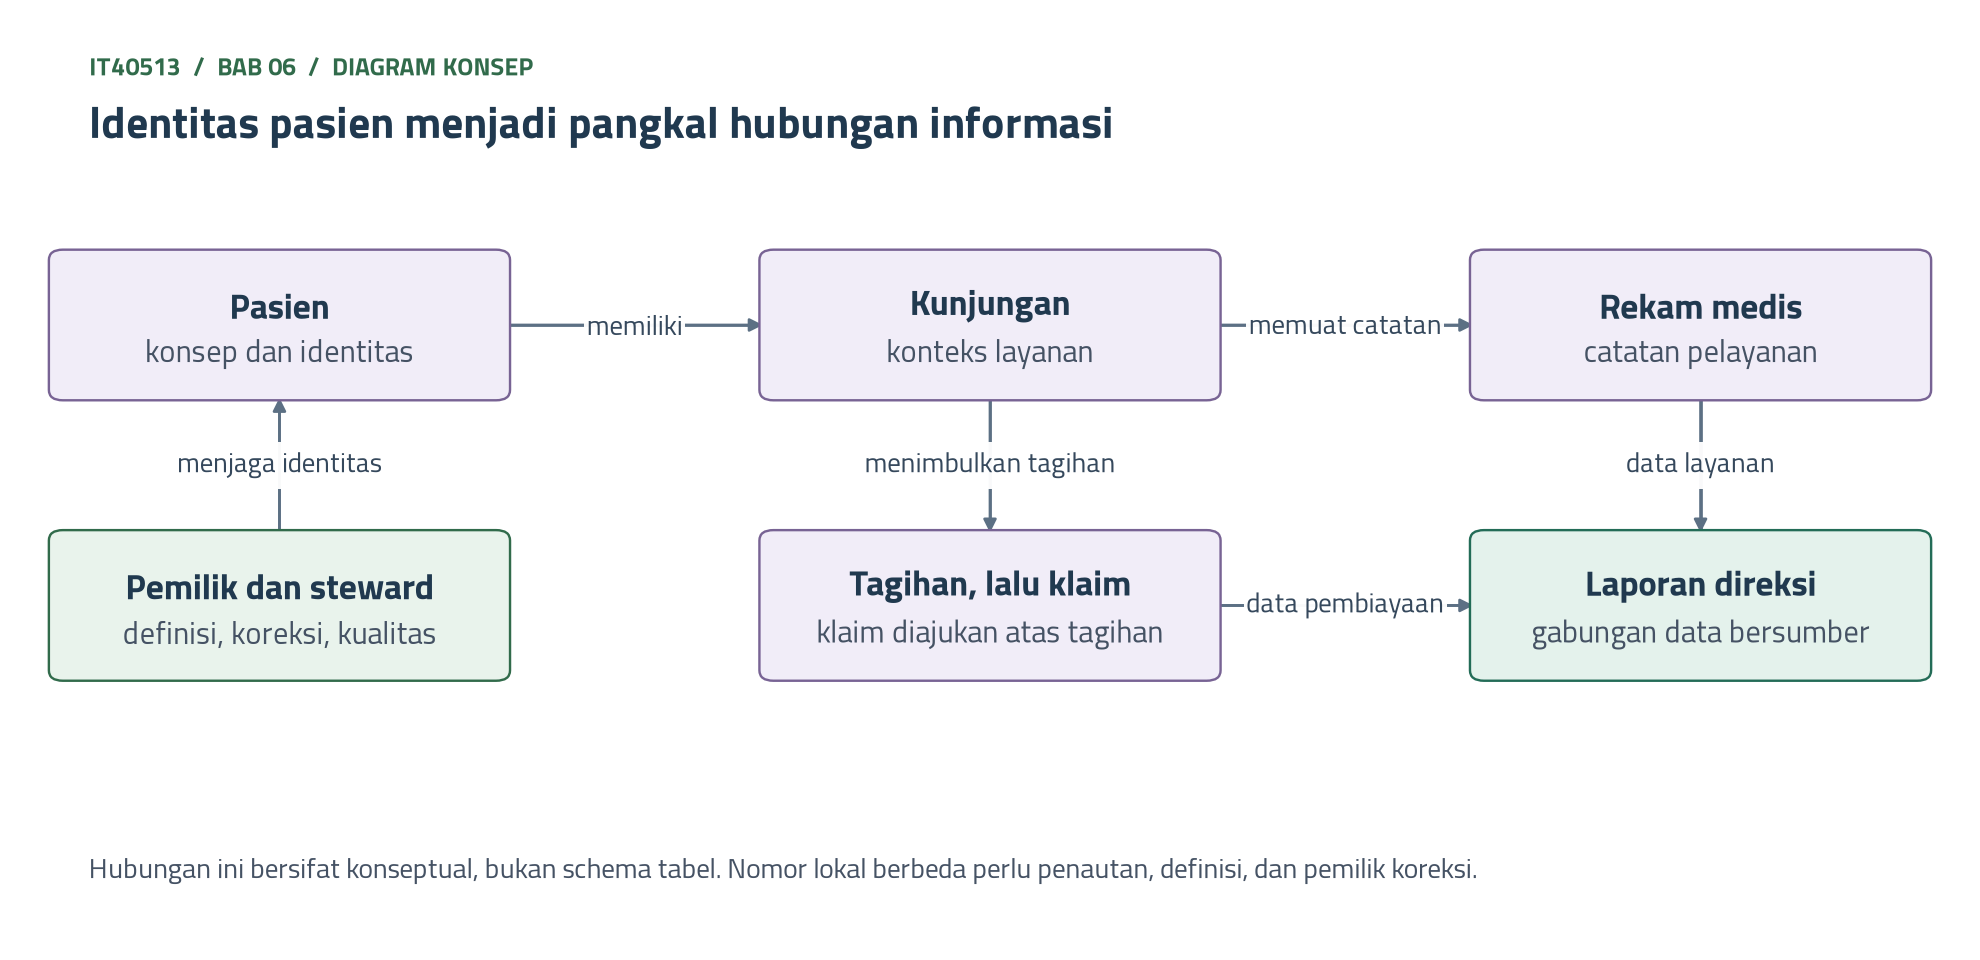
\includegraphics[width=\textwidth]{../figures/ch06-diagram-konsep.png}
  \caption{Identitas pasien menjadi pangkal hubungan informasi}
  \label{fig:ch06-ilustrasi-bab}
\end{figure}
}{}

\section{Konsep Informasi Bisnis dan Model Data Konseptual}

Pertanyaan pertama dalam memotret data bukan "tabel apa saja yang ada di basis
data", melainkan "hal apa saja yang perlu diketahui organisasi agar dapat
bekerja". Pertanyaan pertama hanya dapat dijawab tim TI (Teknologi
Informasi). Pertanyaan kedua
dapat dijawab seluruh tim, termasuk anggota berlatar bisnis, hukum, dan
kesehatan.

\subsection*{Data, informasi, dan konsep bisnis}

Tiga istilah pada bagian ini sering tertukar. Pembagiannya begini. Data adalah
nilai yang tercatat, misalnya angka 38,5 di kolom suhu. Informasi adalah data
yang diberi konteks sehingga dapat dipakai untuk memutuskan, misalnya suhu
seorang pasien anak 38,5 derajat Celsius pukul 08.00, naik dari 37,2 derajat
pada malam sebelumnya. Konsep bisnis adalah hal yang dibicarakan organisasi
dengan arti yang disepakati, misalnya Pasien atau Kunjungan. Tabel
\ref{tab:ch06-data-informasi} merangkum ketiganya.

\begin{table}[!htb]
  \centering
  \caption{Data, informasi, dan konsep bisnis dengan contoh dari Medikara}
  \label{tab:ch06-data-informasi}
  \begin{tabularx}{\textwidth}{lXX}
    \hline
    \textbf{Istilah} & \textbf{Pengertian} & \textbf{Contoh di Medikara} \\
    \hline
    Data & Nilai yang tercatat, belum bermakna tanpa konteks & Angka 38,5; teks
      JKT-0045821 \\
    \hline
    Informasi & Data yang diberi konteks sehingga dapat dipakai untuk memutuskan &
      Suhu pasien anak naik dari 37,2 menjadi 38,5 derajat dalam 10 jam \\
    \hline
    Konsep bisnis & Hal yang dibicarakan organisasi dengan arti yang disepakati &
      Pasien, Kunjungan, Rekam Medis, Klaim \\
    \hline
  \end{tabularx}
\end{table}

Arsitektur data bekerja pada tingkat konsep bisnis. BIZBOK menempatkan
informasi sebagai salah satu ranah inti arsitektur bisnis, sejajar dengan
kapabilitas, \textit{value stream}, dan organisasi \cite{bizbok15}. Satu
konsep informasi (\textit{information concept}) adalah hal yang perlu diketahui
organisasi untuk menjalankan kapabilitasnya. Kumpulan konsep beserta
hubungannya disebut peta informasi (\textit{information map}). Peta ini juga
mencatat tipe dan keadaan tiap konsep. Contohnya, konsep Klaim punya keadaan
diajukan, diverifikasi, dikembalikan, dan dibayar. Keadaan itu penting, karena
laporan "klaim tertunda" hanya bermakna bila semua pihak sepakat kapan sebuah
klaim dianggap tertunda.

Analoginya seperti bagian definisi pada kontrak sewa rumah. Sebelum pasal-pasal
dibaca, kedua pihak menyepakati dulu arti "penyewa", "bangunan", dan "masa
sewa". Tanpa bagian itu, pasal yang sama dibaca berbeda oleh pemilik rumah dan
penyewa, dan perselisihan muncul justru saat keadaan sedang sulit. Peta
informasi adalah bagian definisi itu bagi seluruh organisasi.

Dua contoh kasus nyata dari Medikara memperlihatkan akibatnya bila definisi
belum disepakati:

\begin{enumerate}
  \item Konsep Kunjungan. SIMRS Jakarta mencatat satu kunjungan untuk tiap
        poliklinik yang didatangi, sedangkan SIMRS Bandung mencatat satu
        kunjungan per pasien per hari. Rekap \textit{spreadsheet} juga menghitung
        telekonsultasi Medikara+ sebagai kunjungan. Selisih 2.770 kunjungan pada
        Oktober 2025 berasal dari dua sumber itu: 1.980 telekonsultasi dan 790
        kunjungan ke lebih dari satu poliklinik pada hari yang sama.
  \item Konsep Pasien. Satu akun Medikara+ dapat mendaftarkan sampai lima
        anggota keluarga. Laporan bulanan vendor menyebut "pengguna", sedangkan
        tim pemasaran membacanya sebagai "pasien". Akibatnya, target "pasien
        digital" ditetapkan dari angka akun, padahal satu akun dapat mewakili
        lima orang.
\end{enumerate}

\subsection*{Model data konseptual dalam bahasa bisnis}

Model data konseptual menggambarkan konsep bisnis dan hubungan antarkonsep,
tanpa kolom, tipe data, atau nama tabel. Setiap hubungan ditulis sebagai
kalimat yang dapat dibaca orang bisnis: "Pasien menjalani Kunjungan",
"Kunjungan berlangsung di Fasilitas". Angka di dekat hubungan menyatakan
banyaknya, misalnya satu pasien menjalani banyak kunjungan. Model ini
berbeda dari model data logis yang menambahkan atribut dan kunci, dan dari
model fisik yang menyatakan tabel di basis data tertentu. Gambar
\ref{fig:ch06-model-konseptual} memperlihatkan model konseptual inti Medikara.

\begin{figure}[!htb]
  \centering
  \begin{tikzpicture}[
  font=\scriptsize,
  konsep/.style={draw, rounded corners, minimum height=0.85cm, minimum width=2.4cm,
                 align=center, font=\scriptsize\bfseries},
  panah/.style={-{Stealth[length=2mm]}, thick},
  hubungan/.style={font=\tiny, fill=white, inner sep=1pt, align=center}
]
  \node[konsep, fill=blue!8] (penjamin) at (0,1.8) {Penjamin\\{\tiny\mdseries BPJS, asuransi}};
  \node[konsep, fill=blue!8] (fasilitas) at (4.3,1.8) {Fasilitas\\{\tiny\mdseries RS, klinik, apotek}};
  \node[konsep, fill=blue!8] (dokter) at (8.6,1.8) {Dokter};

  \node[konsep, fill=praditagreen!15] (pasien) at (0,0) {Pasien};
  \node[konsep, fill=orange!12] (kunjungan) at (4.3,0) {Kunjungan};
  \node[konsep, fill=blue!8] (rekam) at (8.6,0) {Rekam Medis};

  \node[konsep, fill=blue!8] (klaim) at (0,-1.8) {Klaim};
  \node[konsep, fill=blue!8] (tagihan) at (4.3,-1.8) {Tagihan};
  \node[konsep, fill=blue!8] (resep) at (8.6,-1.8) {Resep};

  \draw[panah] (pasien) -- node[hubungan] {menjalani\\1 : banyak} (kunjungan);
  \draw[panah] (kunjungan) -- node[hubungan] {berlangsung di} (fasilitas);
  \draw[panah] (kunjungan) -- node[hubungan] {ditangani} (dokter);
  \draw[panah] (kunjungan) -- node[hubungan] {dicatat dalam} (rekam);
  \draw[panah] (rekam) -- node[hubungan] {memuat} (resep);
  \draw[panah] (kunjungan) -- node[hubungan] {ditagihkan lewat} (tagihan);
  \draw[panah] (tagihan) -- node[hubungan] {diajukan sebagai} (klaim);
  \draw[panah] (pasien) -- node[hubungan] {dijamin oleh} (penjamin);
  \draw[panah] (klaim.west) -- ++(-0.45,0) |- node[hubungan, pos=0.25] {dibayar\\oleh}
    (penjamin.west);
\end{tikzpicture}

  \caption{Model data konseptual inti Medikara. Pasien adalah konsep induk, dan
           Kunjungan menjadi titik temu hampir semua konsep lain}
  \label{fig:ch06-model-konseptual}
\end{figure}

Gambar tersebut dibaca dari tengah. Hampir setiap konsep bergantung pada
Kunjungan: rekam medis bertambah karena ada kunjungan, tagihan muncul karena
ada kunjungan, dan klaim diajukan atas tagihan itu. Kunjungan sendiri
bergantung pada Pasien. Artinya, kesalahan pada identitas pasien merambat ke
seluruh rantai di sebelah kanannya. Pengamatan ini menjadi alasan seksi
berikutnya menaruh identitas pasien sebagai data induk terpenting.

\subsection*{Business object dan data object di ArchiMate}

Bab 4 sudah memperkenalkan ArchiMate. Untuk data, tiga elemen struktur pasif
dipakai bersama \cite{archimate32}. \textit{Business object} mewakili konsep
bisnis di lapisan bisnis, misalnya Rekam Medis. \textit{Data object} mewakili
data yang diolah satu aplikasi di lapisan aplikasi, misalnya data rekam medis
di SIMRS Jakarta. \textit{Artifact} mewakili wujud fisiknya di lapisan
teknologi, misalnya basis data atau berkas. Ketiganya dihubungkan dengan relasi
realisasi (\textit{realization}): \textit{data object} merealisasikan
\textit{business object}, dan \textit{artifact} merealisasikan \textit{data
object}. Mata kuliah ini memakai istilah ArchiMate 3.2 karena versi itulah yang
didukung Archi.

Gambar \ref{fig:ch06-objek-archimate} memperlihatkan hasilnya untuk konsep
Rekam Medis. Satu \textit{business object} direalisasikan oleh enam
\textit{data object}: lima di SIMRS dan satu di Medikara+. Tiga di antaranya
digambar sebagai satu kotak "tiga SIMRS lain" agar gambar tetap terbaca.

\begin{figure}[!htb]
  \centering
  \begin{tikzpicture}[
  font=\scriptsize,
  objek/.style={draw, minimum height=0.95cm, minimum width=2.3cm, text width=2.1cm,
                align=center, font=\scriptsize},
  lapisan/.style={font=\scriptsize\bfseries, anchor=east, align=right},
  realisasi/.style={-{Triangle[open, length=2mm, width=2mm]}, thick, dashed}
]
  \node[lapisan] at (-1.4,2.3) {Bisnis};
  \node[lapisan] at (-1.4,0.4) {Aplikasi};
  \node[lapisan] at (-1.4,-1.5) {Teknologi};

  \node[objek, fill=praditagreen!15, font=\scriptsize\bfseries, minimum width=3.0cm,
        text width=2.8cm] (bisnis) at (3.9,2.3)
    {Rekam Medis\\{\tiny\mdseries \textit{business object}}};

  \node[objek, fill=blue!8] (jkt) at (0,0.4)
    {Data rekam medis\\SIMRS Jakarta};
  \node[objek, fill=blue!8] (bks) at (2.6,0.4)
    {Data rekam medis\\SIMRS Bekasi};
  \node[objek, fill=blue!8] (lain) at (5.2,0.4)
    {Data rekam medis\\tiga SIMRS lain};
  \node[objek, fill=orange!12] (vendor) at (7.8,0.4)
    {Catatan\\telekonsultasi\\Medikara+};

  \node[objek, fill=blue!8] (dbjkt) at (0,-1.5)
    {Basis data\\{\tiny on-premise Jakarta}};
  \node[objek, fill=blue!8] (dbbks) at (2.6,-1.5)
    {Basis data\\{\tiny on-premise Bekasi}};
  \node[objek, fill=blue!8] (dblain) at (5.2,-1.5)
    {Tiga basis data\\{\tiny on-premise lain}};
  \node[objek, fill=red!22] (dbvendor) at (7.8,-1.5)
    {Basis data vendor\\{\tiny di luar Medikara}};

  \foreach \objek in {jkt, bks, lain, vendor} {
    \draw[realisasi] (\objek.north) -- (bisnis.south);
  }
  \draw[realisasi] (dbjkt) -- (jkt);
  \draw[realisasi] (dbbks) -- (bks);
  \draw[realisasi] (dblain) -- (lain);
  \draw[realisasi] (dbvendor) -- (vendor);

  \node[font=\tiny, gray, anchor=west] at (-2.4,-2.45)
    {garis putus-putus berujung segitiga terbuka: relasi realisasi};
\end{tikzpicture}

  \caption{Satu \textit{business object} Rekam Medis direalisasikan oleh enam
           \textit{data object} di lima SIMRS dan Medikara+. Kotak merah menandai
           penyimpanan di luar kendali Medikara}
  \label{fig:ch06-objek-archimate}
\end{figure}

Model seperti ini langsung menjawab pertanyaan yang sulit dijawab lewat
wawancara: "di mana saja rekam medis seorang pasien tersimpan?". Jawabannya
enam tempat, dan salah satunya berada di basis data vendor. Jawaban itu kelak
menjadi penting ketika seksi klasifikasi data membahas insiden kebocoran lewat
vendor.

\begin{kasus}[title={Kasus Medikara Health: Enam Konsep Inti}]
  Tim arsitektur Medikara memulai peta informasi dari enam konsep yang paling
  sering muncul di keluhan dan temuan audit. Definisi satu kalimat ditulis
  bersama perwakilan pelayanan medis, keuangan, dan TI, lalu disepakati
  sebagai rujukan untuk seluruh dokumen.

  \begin{enumerate}
    \item \textbf{Pasien}: orang yang terdaftar untuk menerima layanan
          kesehatan di fasilitas Medikara, terlepas dari jumlah akun atau
          nomor yang dimilikinya.
    \item \textbf{Kunjungan}: satu peristiwa pelayanan pada satu fasilitas pada
          satu hari, termasuk telekonsultasi, dengan jenis rawat jalan, rawat
          inap, gawat darurat, atau telekonsultasi.
    \item \textbf{Rekam Medis}: kumpulan catatan klinis seorang pasien dari
          seluruh kunjungannya.
    \item \textbf{Resep}: perintah dokter untuk pemberian obat dalam satu
          kunjungan.
    \item \textbf{Tagihan}: rincian biaya satu kunjungan yang harus dibayar
          pasien atau penjaminnya.
    \item \textbf{Klaim}: permintaan pembayaran atas tagihan kepada penjamin,
          yaitu BPJS (Badan Penyelenggara Jaminan Sosial) Kesehatan atau
          perusahaan asuransi.
  \end{enumerate}

  Definisi Kunjungan sengaja ditulis paling rinci, karena konsep inilah yang
  memicu selisih angka di rapat direksi. Dengan definisi ini, kunjungan ke dua
  poliklinik pada hari yang sama dihitung satu, dan telekonsultasi dihitung
  sebagai jenis kunjungan tersendiri. Tim lalu menambahkan Dokter, Fasilitas,
  dan Penjamin sehingga peta informasi berisi sembilan konsep, seperti pada
  Gambar \ref{fig:ch06-model-konseptual}.
\end{kasus}

\section{Data Induk, Kepemilikan, dan Stewardship}

Pertanyaan kemudian muncul: siapa yang boleh mengubah alamat seorang pasien?
Di Medikara saat ini jawabannya banyak pihak: petugas pendaftaran di lima
rumah sakit, petugas klinik pratama, operator layanan pelanggan Medikara+, dan
pasien sendiri lewat aplikasi. Ketika alamat di dua sistem berbeda, tidak ada
yang tahu versi mana yang benar, dan tidak ada yang merasa wajib
memperbaikinya.

\subsection*{Data induk, data referensi, dan data transaksi}

Tidak semua data perlu dijaga dengan cara yang sama. DAMA-DMBOK membedakan
data menurut perannya \cite{dmbok2}. Data induk (\textit{master data})
adalah data tentang entitas inti yang menjadi konteks bagi banyak transaksi,
dipakai banyak proses, dan berumur panjang. Data referensi (\textit{reference
data}) adalah daftar nilai baku untuk mengelompokkan data lain. Data transaksi
mencatat kejadian pada satu waktu, dan jumlahnya terus bertambah. Tabel
\ref{tab:ch06-jenis-data} memberi contohnya.

\begin{table}[!htb]
  \centering
  \caption{Tiga jenis data menurut perannya, dengan contoh Medikara}
  \label{tab:ch06-jenis-data}
  \begin{tabularx}{\textwidth}{lXXX}
    \hline
    \textbf{Jenis} & \textbf{Ciri} & \textbf{Contoh} & \textbf{Akibat bila salah} \\
    \hline
    Data induk & Entitas inti, dipakai banyak proses, jarang berubah &
      Pasien, Dokter, Fasilitas & Menyebar ke semua transaksi yang merujuknya \\
    \hline
    Data referensi & Daftar nilai baku untuk mengelompokkan data lain &
      Jenis penjamin, kode poliklinik, kode wilayah &
      Laporan tidak dapat dijumlahkan lintas rumah sakit \\
    \hline
    Data transaksi & Catatan kejadian, jumlahnya terus bertambah &
      Kunjungan, Resep, Tagihan, Klaim & Terbatas pada kejadian itu \\
    \hline
  \end{tabularx}
\end{table}

Analoginya seperti administrasi sebuah sekolah. Buku induk siswa adalah data
induk: dibuat sekali saat siswa masuk, lalu dirujuk oleh semua catatan lain.
Daftar kode mata pelajaran adalah data referensi: pendek, jarang berubah, tetapi
tanpa kode yang sama dua kelas tidak dapat dibandingkan. Lembar presensi harian
adalah data transaksi: bertambah setiap hari, dan satu lembar yang salah tidak
merusak lembar lain. Kesalahan nama di buku induk lain ceritanya, karena
kesalahan itu ikut tercetak di rapor, ijazah, dan surat keterangan.

Identitas pasien adalah data induk paling penting di Medikara karena posisinya
di pangkal rantai pada Gambar \ref{fig:ch06-model-konseptual}. Skalanya mudah
dihitung. Medikara melayani sekitar 1,2 juta kunjungan per tahun. Bila tiap
kunjungan menghasilkan rata-rata empat catatan, yaitu kunjungan, catatan
klinis, resep, dan tagihan, maka sekitar 4,8 juta catatan per tahun bergantung
pada benar tidaknya satu data induk: identitas pasien.

\subsection*{Pemilik bisnis, steward, dan pengelola teknis}

Dua hal pada kepemilikan data sering tertukar. Pembagiannya begini. Pemilik
bisnis (\textit{data owner}) adalah pejabat di sisi bisnis yang memutuskan arti
sebuah konsep, mutu minimum yang dapat diterima, dan siapa yang boleh
mengaksesnya. Pengelola teknis (\textit{data custodian}) menjalankan keputusan
itu: menyimpan, mencadangkan, dan memasang hak akses. Bagian TI biasanya
pengelola, bukan pemilik. Ketika bagian TI dianggap pemilik, keputusan
seperti "siapa boleh melihat hasil laboratorium" diambil oleh orang yang tidak
memikul akibat klinis maupun hukumnya.

Di antara keduanya ada peran \textit{data steward}, yaitu orang bisnis yang
menjaga mutu data sehari-hari: menjawab pertanyaan definisi, memperbaiki data
yang salah, dan memeriksa calon duplikat. Tabel \ref{tab:ch06-peran-data}
merangkum ketiga peran untuk konsep Pasien.

\begin{table}[!htb]
  \centering
  \caption{Tiga peran dalam kepemilikan data untuk konsep Pasien di Medikara}
  \label{tab:ch06-peran-data}
  \begin{tabularx}{\textwidth}{lXX}
    \hline
    \textbf{Peran} & \textbf{Tanggung jawab} & \textbf{Untuk konsep Pasien} \\
    \hline
    Pemilik bisnis & Memutuskan definisi, mutu minimum, dan hak akses &
      Saat ini direktur tiap rumah sakit, sehingga ada lima pemilik \\
    \hline
    \textit{Data steward} & Menjaga mutu sehari-hari, memperbaiki data, memeriksa
      calon duplikat & Kepala pendaftaran tiap rumah sakit \\
    \hline
    Pengelola teknis & Menyimpan, mencadangkan, dan memasang hak akses sesuai
      keputusan pemilik & Tim TI tiap rumah sakit, vendor SIMRS, dan vendor
      Medikara+ \\
    \hline
  \end{tabularx}
\end{table}

Khatri dan Brown merumuskan tata kelola data sebagai soal hak memutuskan:
siapa yang berwenang dan siapa yang bertanggung jawab atas keputusan tentang
data. Mereka membaginya ke dalam lima ranah keputusan, yaitu prinsip data,
kualitas data, metadata, akses data, dan siklus hidup data
\cite{c06-khatri2010}. Pada tahap memotret kondisi saat ini, yang dicari adalah
jawaban jujur untuk tiap ranah: siapa yang saat ini memutuskan, walaupun
jawabannya "tidak ada". Rancangan struktur tata kelola datanya dibahas rinci di
mata kuliah IT40813.

\textit{Stewardship} berbeda dari proyek pembersihan data yang dijalankan
sekali. Dua contoh kegiatan \textit{steward} di Medikara:

\begin{enumerate}
  \item Setiap Senin, kepala pendaftaran rumah sakit (RS) Bekasi menerima
        daftar pasien baru
        minggu lalu yang nama dan tanggal lahirnya mirip dengan pasien lama.
        Dari rata-rata 60 calon duplikat per minggu, sekitar 25 terbukti orang
        yang sama dan digabungkan.
  \item Ketika BPJS Kesehatan mengubah aturan jenis kepesertaan,
        \textit{steward} data referensi di kantor pusat memperbarui daftar kode jenis penjamin
        sekali, lalu mengumumkannya ke lima rumah sakit. Tanpa peran itu, tiap
        rumah sakit mengubah kodenya sendiri pada waktu yang berbeda.
\end{enumerate}

Gambar \ref{fig:ch06-identitas-ganda} memperlihatkan akibat bila data induk
pasien tidak punya satu pemilik dan satu kunci penghubung.

\begin{figure}[!htb]
  \centering
  \begin{tikzpicture}[
  font=\scriptsize,
  kotak/.style={draw, rounded corners, minimum height=0.9cm, minimum width=2.6cm,
                align=center, font=\scriptsize\bfseries},
  panah/.style={-{Stealth[length=2mm]}, thick}
]
  \node[kotak, fill=praditagreen!15] (orang) at (0,0)
    {Satu orang\\{\tiny\mdseries Ibu Ratna, fiktif}};

  \node[kotak, fill=blue!8] (jkt) at (4.0,1.4)
    {RS Jakarta\\{\tiny\mdseries nomor JKT-0045821}\\{\tiny\mdseries riwayat diabetes}};
  \node[kotak, fill=blue!8] (bks) at (4.0,0)
    {RS Bekasi\\{\tiny\mdseries nomor BKS-118204}\\{\tiny\mdseries alergi penisilin}};
  \node[kotak, fill=orange!12] (app) at (4.0,-1.4)
    {Medikara+\\{\tiny\mdseries akun M-77120}\\{\tiny\mdseries telekonsultasi 2025}};

  \node[kotak, fill=gray!35] (tanpa) at (8.3,0)
    {Tiga catatan,\\tanpa kunci\\penghubung};
  \node[kotak, fill=red!22] (alergi) at (8.3,1.6)
    {Alergi tidak terlihat\\{\tiny\mdseries oleh dokter di Jakarta}};
  \node[kotak, fill=red!22] (hitung) at (8.3,-1.6)
    {Dihitung sebagai\\{\tiny\mdseries tiga pasien berbeda}};

  \draw[panah] (orang.east) -- ++(0.5,0) |- (jkt.west);
  \draw[panah] (orang.east) -- (bks.west);
  \draw[panah] (orang.east) -- ++(0.5,0) |- (app.west);
  \draw[panah] (jkt.east) -- (tanpa.west);
  \draw[panah] (bks.east) -- (tanpa.west);
  \draw[panah] (app.east) -- (tanpa.west);
  \draw[panah] (tanpa) -- (alergi);
  \draw[panah] (tanpa) -- (hitung);
\end{tikzpicture}

  \caption{Satu orang tercatat dengan tiga nomor di tiga tempat. Tanpa kunci
           penghubung, riwayat klinisnya terpecah dan laporan menghitungnya
           sebagai tiga pasien}
  \label{fig:ch06-identitas-ganda}
\end{figure}

\begin{kasus}[title={Kasus Medikara Health: Lima Pola Nomor Rekam Medis}]
  Kelima rumah sakit Medikara berasal dari akuisisi, dan masing-masing membawa
  pola nomor rekam medis sendiri, misalnya \texttt{JKT-0045821} di Jakarta dan
  \texttt{BKS-118204} di Bekasi. Klinik pratama memakai nomor dari SIMRS rumah
  sakit induk di wilayahnya, sedangkan Medikara+ memberi nomor akun sendiri.
  Tidak ada satu kunci pun yang menghubungkan semua nomor itu. Nomor Induk
  Kependudukan (NIK) memang tersimpan, tetapi kolomnya tidak wajib diisi pada
  pendaftaran sebelum 2020.

  Misalkan tim arsitektur mengambil sampel acak 10.000 nomor rekam medis aktif
  dari kelima SIMRS, lalu mencocokkan NIK, nama, dan tanggal lahirnya.
  Hasilnya 1.140 nomor, atau 11,4 persen, ternyata milik orang yang sudah
  punya nomor di rumah sakit lain.

  Temuan ini punya dua konsekuensi. Pertama, dokter di satu rumah sakit tidak
  melihat riwayat yang tercatat di rumah sakit lain, seperti alergi penisilin
  Ibu Ratna pada Gambar \ref{fig:ch06-identitas-ganda}. Kedua, setiap laporan
  "jumlah pasien" yang menjumlahkan lima SIMRS menghitung orang yang sama lebih
  dari sekali. Pemilik bisnis konsep Pasien saat ini ada lima orang, yaitu
  direktur tiap rumah sakit, sehingga tidak ada yang berwenang menetapkan satu
  aturan penomoran untuk seluruh jaringan. Temuan kepemilikan inilah yang
  dicatat untuk C2, sedangkan rancangan identitas pasien tunggal dikerjakan di
  Bab 9.
\end{kasus}

\section{Lokasi dan Aliran Data}

Setiap awal bulan, dua staf perencanaan Medikara mengunduh tujuh ekspor: satu
dari tiap SIMRS, satu dari ERP, dan satu dari Medikara+. Ekspor baru dapat
diambil setelah tutup buku pada hari kerja kelima. Ketujuhnya digabung di
\textit{spreadsheet} selama enam hari kerja, lalu disetujui, sehingga laporan
direksi terbit pada hari kerja ke-12. Pekerjaan ini menghabiskan 12 hari-orang
per bulan, atau 144 hari-orang per tahun. Aliran ini tidak tercatat di diagram
integrasi mana pun, padahal angka direksi bergantung sepenuhnya padanya.

\subsection*{Aliran data tingkat tinggi}

Diagram aliran data tingkat tinggi menggambarkan di mana sebuah konsep dibuat,
ke mana disalin, dan siapa yang memakainya, tanpa rincian kolom atau protokol.
TOGAF menyebut gambaran semacam ini \textit{Data Dissemination diagram}, dan
melengkapinya dengan katalog entitas data serta \textit{Application/Data
matrix} yang memetakan aplikasi ke data \cite{togaf10}. Yang digambar adalah
aliran yang sungguh terjadi, termasuk aliran manual, bukan aliran yang
seharusnya terjadi menurut dokumen proyek.

Analoginya seperti peta saluran air di sebuah perumahan. Peta resmi dari
pengembang memperlihatkan pipa dari tandon ke tiap rumah. Selang yang dipasang
warga sendiri untuk menyiram taman tetangga tidak ada di peta itu, padahal di
sanalah kebocoran paling sering terjadi. Rekap \textit{spreadsheet} adalah selang
yang dipasang sendiri itu.

Gambar \ref{fig:ch06-aliran-data} memperlihatkan aliran data tingkat tinggi
Medikara saat ini.

\begin{figure}[!htb]
  \centering
  \begin{tikzpicture}[
  font=\scriptsize,
  kotak/.style={draw, rounded corners, minimum height=0.9cm, minimum width=2.5cm,
                align=center, font=\scriptsize\bfseries},
  luar/.style={kotak, dashed, fill=blue!8},
  panah/.style={-{Stealth[length=2mm]}, thick},
  manual/.style={-{Stealth[length=2mm]}, thick, dashed, red!65!black},
  label/.style={font=\tiny, fill=white, inner sep=1pt, align=center}
]
  \node[kotak, fill=blue!8] (mplus) at (0,1.8)
    {Medikara+\\{\tiny\mdseries janji temu, telekonsultasi}};
  \node[kotak, fill=praditagreen!15] (simrs) at (0,0)
    {5 SIMRS\\{\tiny\mdseries RS, klinik, lab, apotek}};
  \node[kotak, fill=blue!8] (erp) at (0,-1.8)
    {ERP keuangan\\{\tiny\mdseries terpusat}};

  \node[luar] (bpjs) at (4.6,2.0) {BPJS Kesehatan\\{\tiny\mdseries eksternal}};
  \node[luar] (satu) at (4.6,0.7) {SATUSEHAT\\{\tiny\mdseries eksternal}};
  \node[kotak, fill=red!22] (sheet) at (4.6,-1.0)
    {Spreadsheet\\{\tiny\mdseries rekap bulanan}};
  \node[kotak, fill=green!10] (laporan) at (8.9,-1.0)
    {Laporan\\manajemen};

  \draw[panah, {Stealth[length=2mm]}-{Stealth[length=2mm]}] (mplus) --
    node[label] {janji temu, jadwal} (simrs);
  \draw[panah] (simrs) -- node[label] {tagihan} (erp);
  \draw[panah] ([yshift=0.2cm]simrs.east) -- ++(0.9,0) |-
    node[label, pos=0.75] {klaim} (bpjs.west);
  \draw[panah] ([yshift=0.2cm]simrs.east) -- ++(0.9,0) |-
    node[label, pos=0.75] {kunjungan} (satu.west);
  \draw[manual] ([yshift=-0.2cm]simrs.east) -- ++(0.6,0) |-
    node[label, pos=0.75] {ekspor} (sheet.west);
  \draw[manual] (erp.east) -- ++(0.6,0) |- (sheet.west);
  \draw[manual] (sheet) -- node[label] {salin dan tempel} (laporan);

  \node[font=\tiny, gray, anchor=west] at (6.6,-2.3)
    {garis merah putus-putus:};
  \node[font=\tiny, gray, anchor=west] at (6.6,-2.6)
    {aliran manual yang tidak tercatat};
\end{tikzpicture}

  \caption{Aliran data tingkat tinggi Medikara saat ini. Integrasi resmi ke BPJS
           Kesehatan dan SATUSEHAT tercatat, sedangkan aliran ke laporan
           manajemen berjalan manual lewat \textit{spreadsheet}}
  \label{fig:ch06-aliran-data}
\end{figure}

Dua hal terbaca dari gambar tersebut. Pertama, SIMRS menjadi sumber hampir
semua aliran, sehingga perbedaan versi di lima SIMRS langsung terbawa ke BPJS
Kesehatan, SATUSEHAT, dan laporan. Kedua, satu-satunya jalan dari data
operasional ke laporan manajemen adalah jalur merah, yang tidak punya kontrol
akses, riwayat perubahan, maupun pemilik. Rincian integrasi SIMRS ke BPJS
Kesehatan dan SATUSEHAT dibahas di Bab 7 dan di mata kuliah IT40613.

\subsection*{Matriks CRUD antara data dan aplikasi}

Diagram aliran memperlihatkan arah, tetapi belum memperlihatkan peran tiap
aplikasi. Matriks CRUD mengisi kekosongan itu. Baris matriks berisi konsep
data, kolomnya berisi aplikasi, dan tiap sel berisi huruf yang menyatakan apa
yang dilakukan aplikasi itu terhadap konsep tersebut: C (\textit{create}) membuat,
R (\textit{read}) membaca, U (\textit{update}) mengubah, dan D (\textit{delete})
menghapus. Sel kosong berarti aplikasi itu tidak menyentuh konsep tersebut.
Matriks ini adalah bentuk sederhana dari \textit{Application/Data matrix} dalam
TOGAF \cite{togaf10}.

Tabel \ref{tab:ch06-crud} memuat matriks CRUD Medikara saat ini. Kolom SIMRS
mewakili lima aplikasi terpisah yang mengerjakan hal yang sama, dan kolom
\textit{spreadsheet} sengaja ditulis sebagai aplikasi tersendiri.

\begin{table}[!htb]
  \centering
  \caption{Matriks CRUD Medikara saat ini, tersedia di
           \berkas{sources/chapter06/medikara-matriks-crud.csv}}
  \label{tab:ch06-crud}
  \begin{tabularx}{\textwidth}{Xcccc}
    \hline
    \textbf{Konsep} & \textbf{SIMRS (5)} & \textbf{Medikara+} & \textbf{ERP} &
      \textbf{\textit{Spreadsheet}} \\
    \hline
    Pasien & CRU & CRU & R & R \\
    \hline
    Janji Temu & RU & CRUD & & \\
    \hline
    Kunjungan & CRU & CR & & R \\
    \hline
    Rekam Medis & CRU & CR & & \\
    \hline
    Hasil Laboratorium & CRU & R & & R \\
    \hline
    Resep & CRU & R & & \\
    \hline
    Jadwal Praktik Dokter & CRUD & R & & \\
    \hline
    Tagihan & CRU & R & RU & R \\
    \hline
    Klaim & CRU & & R & CRU \\
    \hline
    Kontrak Penjamin & R & & R & CRUD \\
    \hline
  \end{tabularx}
\end{table}

Matriks dibaca per baris, lalu per pola. Tabel \ref{tab:ch06-pola-crud}
merangkum lima pola yang paling sering menandai masalah.

\begin{table}[!htb]
  \centering
  \caption{Pola pada matriks CRUD dan artinya bagi arsitektur data}
  \label{tab:ch06-pola-crud}
  \begin{tabularx}{\textwidth}{XXX}
    \hline
    \textbf{Pola} & \textbf{Artinya} & \textbf{Contoh di Medikara} \\
    \hline
    C di lebih dari satu kolom & Ada beberapa versi kebenaran yang harus
      disatukan belakangan & Pasien, Kunjungan, Rekam Medis, Klaim \\
    \hline
    C hanya di kolom \textit{spreadsheet} & Data penting di luar aplikasi yang
      dikelola, biasanya tanpa pemilik & Kontrak Penjamin \\
    \hline
    R di kolom \textit{spreadsheet} & Aliran manual yang tidak tercatat di
      diagram integrasi & Pasien, Kunjungan, Hasil Laboratorium, Tagihan \\
    \hline
    Tidak ada D di baris mana pun & Data tidak pernah dihapus, wajar bila
      diwajibkan aturan masa simpan & Rekam Medis, Resep, Tagihan \\
    \hline
    Tidak ada C sama sekali & Data datang dari luar atau masih dicatat di
      kertas & Tidak ditemukan pada contoh ini \\
    \hline
  \end{tabularx}
\end{table}

Pola pertama paling mahal akibatnya. Karena kolom SIMRS mewakili lima
aplikasi, konsep Pasien dibuat di enam tempat: lima SIMRS dan Medikara+. Konsep
Kunjungan juga dibuat di enam tempat, karena telekonsultasi tercatat di
Medikara+, yaitu 1.980 kunjungan pada Oktober 2025. Konsep Rekam Medis juga
dibuat di enam tempat, dan salah satunya adalah catatan telekonsultasi di
Medikara+ yang disimpan vendor. Konsep Klaim
dibuat di SIMRS untuk BPJS Kesehatan, tetapi klaim ke asuransi swasta masih
direkap di \textit{spreadsheet}. Setiap baris dengan lebih dari satu C adalah
calon masalah konsistensi di seksi kualitas data.

Pola kedua menunjukkan data yang tidak punya rumah. Kontrak Penjamin, yaitu
kesepakatan tarif dan syarat dengan BPJS Kesehatan dan 14 perusahaan asuransi,
hanya dibuat dan diubah di satu berkas \textit{spreadsheet} milik bagian
keuangan. SIMRS dan ERP membaca angkanya lewat salinan manual. Matriks ini
juga memperlihatkan bahwa konsep tersebut belum punya pemilik bisnis, dan
temuan itu dibahas lagi di Latihan 2.

\subsection*{Spreadsheet sebagai aliran data tersembunyi}

Huruf R di kolom \textit{spreadsheet} sering dianggap tidak berbahaya karena
"hanya membaca". Anggapan itu keliru karena dua alasan. Pertama, setiap
ekspor membuat salinan data di luar aplikasi, sehingga data pasien ikut
berpindah ke laptop staf, surel, dan folder bersama. Kedua, salinan itu diolah
dengan rumus yang tidak pernah ditinjau. Satu baris rumus yang tergeser cukup
untuk mengubah angka direksi tanpa jejak.

\textit{Spreadsheet} tidak perlu dihapus dari peta. Justru sebaliknya:
\textit{spreadsheet} harus muncul sebagai kolom di matriks CRUD dan sebagai
kotak di diagram aliran, agar biayanya terlihat. Untuk Medikara, biayanya
144 hari-orang per tahun dan laporan yang terlambat 12 hari kerja. Angka itu
menjadi bukti di daftar masalah data, dan kelak menjadi dasar
\textit{business case} di Bab 13.

\begin{pendalaman}
  Matriks CRUD yang berisi 15 konsep dan 10 aplikasi sudah memuat 150 sel.
  Membacanya dengan mata cukup untuk sekali, tetapi tidak cukup bila matriks
  diperbarui setiap kali ada aplikasi baru. Skrip pada Listing
  \ref{lst:ch06-periksa} membaca matriks berformat CSV (\textit{Comma-Separated
  Values}) dan menandai pola pada Tabel \ref{tab:ch06-pola-crud} secara
  otomatis.

  \lstdefinestyle{ch06python}{
    language=Python, basicstyle=\ttfamily\scriptsize,
    keywordstyle=\color{blue}\bfseries, commentstyle=\color{gray}\itshape,
    stringstyle=\color{red}, showstringspaces=false, breaklines=true,
    frame=lines, numbers=left, numberstyle=\tiny\color{gray},
    backgroundcolor=\color{lightgray!10}, tabsize=2, captionpos=b
  }

\begin{lstlisting}[style=ch06python, caption={Pemeriksaan satu baris matriks CRUD, tersedia di \berkas{sources/chapter06/periksa-matriks-crud.py}}, label={lst:ch06-periksa}]
def periksa_satu_konsep(baris):
  """Mengembalikan tanda untuk satu konsep, kosong bila tidak ada."""
  tanda = []
  if not (baris.get(KOLOM_PEMILIK) or "").strip():
    tanda.append("belum punya pemilik bisnis")

  pembuat = aplikasi_dengan_huruf(baris, "C")
  if not pembuat:
    tanda.append("tidak ada aplikasi yang membuatnya")
  elif len(pembuat) > BATAS_JUMLAH_PEMBUAT:
    tanda.append(f"dibuat di {len(pembuat)} tempat: {', '.join(pembuat)}")

  if KOLOM_SPREADSHEET in pembuat:
    tanda.append("dibuat di spreadsheet, di luar aplikasi yang dikelola")
  return tanda
\end{lstlisting}

  Fungsi \texttt{aplikasi\_dengan\_huruf} mengembalikan daftar kolom yang
  selnya memuat satu huruf tertentu. Konsep tanpa huruf D diperiksa oleh
  fungsi terpisah, karena pola itu tidak otomatis salah: rekam medis memang
  wajib disimpan lama. Listing \ref{lst:ch06-periksa-jalan} memuat keluarannya
  apa adanya untuk matriks Medikara.

\begin{lstlisting}[language=bash, caption={Menjalankan pemeriksa pada matriks Medikara, tersedia di \berkas{sources/chapter06/periksa-matriks-crud.py}}, label={lst:ch06-periksa-jalan}]
python periksa-matriks-crud.py medikara-matriks-crud.csv

# Keluarannya:
# Pasien
#   - dibuat di 2 tempat: simrs, medikara_plus
# Kunjungan
#   - dibuat di 2 tempat: simrs, medikara_plus
# Rekam Medis
#   - dibuat di 2 tempat: simrs, medikara_plus
# Klaim
#   - dibuat di 2 tempat: simrs, spreadsheet
#   - dibuat di spreadsheet, di luar aplikasi yang dikelola
# Kontrak Penjamin
#   - belum punya pemilik bisnis
#   - dibuat di spreadsheet, di luar aplikasi yang dikelola
#
# Ditandai: 5 dari 10 konsep.
# Tanpa penghapus, cocokkan dengan aturan masa simpan:
#   Pasien, Kunjungan, Rekam Medis, Hasil Laboratorium, Resep, Tagihan, Klaim
\end{lstlisting}

  Skrip melaporkan "2 tempat" untuk Pasien karena kolom \texttt{simrs} dihitung
  satu. Keterbatasan ini disengaja agar berkasnya tetap sederhana. Tim yang
  ingin melihat angka persisnya cukup memecah kolom itu menjadi lima kolom,
  satu untuk tiap rumah sakit.
\end{pendalaman}

\section{Klasifikasi Data dan Kewajiban Regulasi}

Ketika insiden kebocoran lewat vendor terjadi pada 2025, pertanyaan pertama
direksi sederhana: data apa saja yang bocor, dan seberapa parah? Pertanyaan itu
butuh tiga hari untuk dijawab, karena tidak ada daftar yang menyatakan konsep
mana yang tersimpan di sistem vendor dan seberapa sensitif masing-masing.
Klasifikasi data dibuat agar pertanyaan semacam itu terjawab dalam hitungan
menit.

\subsection*{Skema klasifikasi yang sederhana}

Klasifikasi data adalah pemberian label tingkat sensitivitas pada tiap konsep
data. Aturan penyimpanan, akses, dan berbagi kemudian diturunkan dari label
itu, sehingga tidak perlu diputuskan ulang setiap kali ada proyek baru. Skema
yang baik cukup sederhana agar dapat dipakai petugas pendaftaran, bukan hanya
oleh tim keamanan. Tabel \ref{tab:ch06-klasifikasi} memuat skema empat tingkat
yang dipakai bab ini.

\begin{table}[!htb]
  \centering
  \caption{Skema klasifikasi data empat tingkat dengan contoh Medikara}
  \label{tab:ch06-klasifikasi}
  \begin{tabularx}{\textwidth}{lXXX}
    \hline
    \textbf{Tingkat} & \textbf{Arti} & \textbf{Contoh} & \textbf{Perlakuan
      minimum} \\
    \hline
    Publik & Boleh diketahui siapa pun & Daftar layanan, tarif umum, alamat
      fasilitas & Tanpa pembatasan baca, perubahan lewat pemilik \\
    \hline
    Internal & Untuk karyawan, kerugian kecil bila bocor & SOP (\textit{Standard
      Operating Procedure}), materi pelatihan & Hanya akun karyawan \\
    \hline
    Rahasia & Kerugian nyata bagi organisasi atau orang bila bocor & Identitas
      pasien, laporan pendapatan, kontrak penjamin & Akses menurut peran,
      tercatat, tidak di perangkat pribadi \\
    \hline
    Sangat Rahasia & Kerugian berat, termasuk data pribadi spesifik & Rekam
      medis, diagnosis, catatan telekonsultasi & Akses seperlunya, dienkripsi,
      tiap akses dicatat, berbagi hanya lewat perjanjian \\
    \hline
  \end{tabularx}
\end{table}

Analoginya seperti pembagian ruang di sebuah rumah sakit. Lobi terbuka untuk
siapa pun. Ruang staf hanya untuk karyawan berkartu. Ruang arsip rekam medis
hanya untuk petugas tertentu. Lemari obat golongan narkotika dikunci ganda,
dan setiap pembukaannya dicatat. Tidak ada yang perlu bertanya ulang setiap
hari siapa boleh masuk ke ruang mana, karena aturannya menempel pada ruangnya.

\subsection*{Data pribadi umum dan data pribadi spesifik}

Dua hal pada klasifikasi sering tertukar. Pembagiannya begini. Tingkat
klasifikasi pada Tabel \ref{tab:ch06-klasifikasi} adalah keputusan organisasi
tentang seberapa ketat sebuah data diperlakukan. Kategori data pribadi adalah
ketentuan undang-undang tentang jenis data yang dilindungi. UU 27/2022 Pasal 4
membagi data pribadi menjadi dua \cite{uu27-2022-pdp}. Data pribadi yang
bersifat spesifik meliputi data dan informasi kesehatan, data biometrik, data
genetika, catatan kejahatan, data anak, data keuangan pribadi, dan data lain
sesuai peraturan perundang-undangan. Data pribadi yang bersifat umum meliputi
nama lengkap, jenis kelamin, kewarganegaraan, agama, status perkawinan, dan
data pribadi yang dikombinasikan untuk mengidentifikasi seseorang.

Kedua sumbu itu tidak selalu sejalan. Rencana akuisisi klinik baru tergolong
Rahasia walaupun bukan data pribadi sama sekali. Sebaliknya, nama dokter adalah
data pribadi umum, tetapi tetap dapat tergolong Publik bila memang sengaja
diumumkan untuk melayani pasien. Karena itu katalog konsep informasi mencatat
keduanya dalam dua kolom terpisah. Kewajiban rinci yang muncul dari UU PDP
(Pelindungan Data Pribadi), seperti dasar pemrosesan, hak subjek data, dan
notifikasi kegagalan pelindungan, dibahas di mata kuliah IT40813. Bab ini
hanya memakai kategorinya untuk memberi label.

\subsection*{Kewajiban rekam medis elektronik}

Permenkes 24/2022 menambahkan kewajiban yang langsung membentuk arsitektur
data rumah sakit \cite{permenkes24-2022}. Tabel \ref{tab:ch06-kewajiban}
merangkum ketentuan yang paling berpengaruh beserta akibatnya.

\begin{table}[!htb]
  \centering
  \caption{Ketentuan regulasi yang membentuk arsitektur data Medikara}
  \label{tab:ch06-kewajiban}
  \begin{tabularx}{\textwidth}{lXX}
    \hline
    \textbf{Ketentuan} & \textbf{Isi singkat} & \textbf{Akibat bagi arsitektur
      data} \\
    \hline
    UU 27/2022 Pasal 4 & Data kesehatan dan data keuangan pribadi termasuk data
      pribadi spesifik & Rekam Medis, Hasil Laboratorium, Resep, dan Klaim diberi
      label spesifik \\
    \hline
    Permenkes 24/2022 Pasal 3 ayat (1) & Setiap fasilitas pelayanan kesehatan
      wajib menyelenggarakan rekam medis elektronik & Catatan klinis di kertas
      atau \textit{spreadsheet} tidak memenuhi \\
    \hline
    Pasal 21 & Rekam medis elektronik harus terhubung dengan platform
      interoperabilitas Kementerian Kesehatan & Kelima SIMRS wajib mampu
      mengirim data ke SATUSEHAT \\
    \hline
    Pasal 25 ayat (1) & Dokumen rekam medis milik fasilitas, sedangkan isinya
      milik pasien & Permintaan pasien harus dapat dijawab dari semua tempat
      penyimpanan \\
    \hline
    Pasal 39 ayat (1) & Rekam medis elektronik disimpan paling singkat 25 tahun
      sejak kunjungan terakhir & Data harus bertahan lebih lama daripada
      aplikasinya \\
    \hline
    Pasal 45 & Penyesuaian paling lambat 31 Desember 2023 & Kewajiban sudah
      berlaku penuh \\
    \hline
  \end{tabularx}
\end{table}

Ketentuan masa simpan punya konsekuensi yang mudah terlewat. Bila jumlah
kunjungan tetap 1,2 juta per tahun, dalam 25 tahun Medikara memegang paling
sedikit 30 juta catatan kunjungan yang wajib tetap dapat dibaca. Selama itu
SIMRS hampir pasti berganti dua atau tiga kali. Artinya, data rekam medis
harus dirancang agar dapat berpindah dari satu aplikasi ke aplikasi
berikutnya, dan tidak terkunci di format milik satu vendor. Ketiadaan huruf D
pada baris Rekam Medis di Tabel \ref{tab:ch06-crud} karena itu benar, asalkan
keputusan itu tercatat dan disengaja.

\subsection*{Dampak klasifikasi pada lokasi dan akses}

Label klasifikasi baru berguna bila dipasang pada peta yang sudah dibuat. Dua
contoh dari Medikara:

\begin{enumerate}
  \item Rekap \textit{spreadsheet} bulanan memuat kolom Hasil Laboratorium untuk
        menghitung jumlah pemeriksaan. Karena konsep itu Sangat Rahasia,
        salinannya tidak boleh berada di laptop staf perencanaan. Laporan yang
        hanya membutuhkan jumlah cukup menerima angka agregat, bukan baris
        hasil per pasien.
  \item Medikara+ membuat catatan telekonsultasi, yang termasuk Rekam Medis
        dan tergolong Sangat Rahasia. Basis datanya berada di vendor. Lokasi
        itu tidak otomatis dilarang, tetapi memicu tiga syarat: perjanjian
        pemrosesan dengan vendor, hak akses yang tercatat, dan kemampuan
        mengembalikan seluruh data bila kontrak berakhir.
\end{enumerate}

\begin{kasus}[title={Kasus Medikara Health: Kebocoran Lewat Vendor dari Sudut Pandang Data}]
  Rincian insiden 2025 mengikuti data latihan IT40613 Bab 6. Akun dukungan
  vendor yang masih aktif setelah kontrak selesai memanggil API bawaan SIMRS di
  dua rumah sakit, 155 panggilan per malam selama 8 malam, sehingga 1.240 rekam
  kunjungan terbaca. Medikara baru mengetahuinya pada hari ke-11 lewat keluhan
  pasien, dan hanya 620 rekam yang masih terlacak.

  Dari sudut pandang arsitektur data, insiden ini membuka empat celah yang
  sudah terlihat di artefak bab ini:

  \begin{enumerate}
    \item Gambar \ref{fig:ch06-objek-archimate} memperlihatkan bahwa Rekam
          Medis juga direalisasikan di basis data vendor, tetapi tidak ada
          dokumen Medikara yang mencatatnya sebelum insiden.
    \item Rekam kunjungan memuat data kesehatan, sehingga tergolong data
          pribadi spesifik dan Sangat Rahasia. Label itu belum pernah dipasang,
          sehingga hak akun dukungan tidak dibatasi menurut kelas data.
    \item Tidak ada pemilik bisnis yang berwenang menilai akses akun dukungan
          setelah kontrak pekerjaan selesai.
    \item Aliran dari API bawaan SIMRS ke akun dukungan vendor tidak muncul di
          diagram aliran mana pun, persis seperti aliran \textit{spreadsheet}
          pada Gambar \ref{fig:ch06-aliran-data}.
  \end{enumerate}

  Keempat celah itu dicatat di daftar masalah data untuk C2. Penilaian hukumnya,
  yaitu siapa pengendali, siapa prosesor, dan apakah notifikasi sudah memenuhi
  kewajiban, dibahas di mata kuliah IT40813.
\end{kasus}

\section{Masalah Kualitas Data}

Bagian klaim Medikara menerima berkas yang dikembalikan BPJS Kesehatan
setiap hari karena data tidak cocok. Misalkan 40 persen dari 1,2 juta kunjungan
per tahun dijamin BPJS Kesehatan, sehingga ada sekitar 40.000 berkas klaim per
bulan. Bila 3,5 persen di antaranya dikembalikan, ada 1.400 berkas yang harus
diperbaiki. Dengan 15 menit per berkas, perbaikan itu memakan 350 jam kerja per
bulan, atau sekitar 44 hari kerja. Angka itu setara dua petugas penuh waktu,
belum termasuk pembayaran yang tertunda.

\subsection*{Dimensi kualitas data}

Kualitas data adalah kesesuaian data untuk dipakai oleh pemakainya. Wang dan
Strong menunjukkan bahwa pemakai data menilai kualitas bukan hanya dari
ketepatan nilai, melainkan dari banyak dimensi yang mereka kelompokkan ke
dalam empat kategori: intrinsik, kontekstual, representasional, dan
aksesibilitas \cite{c06-wang1996}. ISO/IEC 25012:2008 merumuskan 15
karakteristik kualitas data dan membaginya menjadi karakteristik yang melekat
pada data serta karakteristik yang bergantung pada sistem penyimpannya
\cite{c06-iso25012}. Standar itu diterbitkan bersama oleh ISO
(\textit{International Organization for Standardization}) dan IEC
(\textit{International Electrotechnical Commission}). Untuk memotret kondisi saat ini, empat dimensi yang
melekat pada data sudah cukup: akurasi, kelengkapan, konsistensi, dan
ketepatan waktu. Bab ini menambahkan keunikan, yang dipakai DAMA-DMBOK untuk
mengukur catatan ganda \cite{dmbok2}.

Analoginya seperti daftar alamat undangan pernikahan. Alamat yang salah tulis
membuat undangan nyasar, dan itu soal akurasi. Nomor rumah yang kosong adalah
soal kelengkapan. Daftar keluarga mempelai pria dan wanita yang mencatat alamat
berbeda untuk tamu yang sama adalah soal konsistensi. Alamat lama milik tamu
yang sudah pindah adalah soal ketepatan waktu. Tamu yang tercatat dua kali
sehingga menerima dua undangan adalah soal keunikan.

Tabel \ref{tab:ch06-kualitas} menerapkan kelima dimensi pada Medikara. Angkanya
adalah hasil pengukuran awal yang diandaikan, dan tiap tim mengukur ulang pada
organisasinya sendiri.

\begin{table}[!htb]
  \centering
  \caption{Lima dimensi kualitas data dengan ukuran awal yang diandaikan di
           Medikara}
  \label{tab:ch06-kualitas}
  \begin{tabularx}{\textwidth}{lXXX}
    \hline
    \textbf{Dimensi} & \textbf{Pertanyaan} & \textbf{Ukuran di Medikara} &
      \textbf{Dampak} \\
    \hline
    Akurasi & Apakah nilainya sesuai kenyataan? & 4,2\% dari 2.000 alamat
      sampel tidak sesuai kartu identitas & Surat hasil pemeriksaan salah
      alamat \\
    \hline
    Kelengkapan & Apakah kolom wajib terisi? & NIK kosong pada 9\% pasien yang
      terdaftar sebelum 2020 & Tidak dapat memperoleh Nomor SATUSEHAT Pasien \\
    \hline
    Konsistensi & Apakah dua sumber sepakat? & Kunjungan Oktober 2025: 99.870
      di SIMRS, 102.640 di laporan & Direksi ragu memakai angka \\
    \hline
    Ketepatan waktu & Apakah data tersedia saat dibutuhkan? & Laporan terbit
      hari kerja ke-12; data ke SATUSEHAT rata-rata 3 hari & Keputusan bulan
      berjalan memakai angka bulan lalu \\
    \hline
    Keunikan & Apakah satu orang tercatat sekali? & 11,4\% dari 10.000 nomor
      rekam medis sampel adalah duplikat lintas rumah sakit & Riwayat klinis
      terpecah, jumlah pasien terlalu besar \\
    \hline
  \end{tabularx}
\end{table}

Baris konsistensi memperlihatkan selisih 2.770 kunjungan, atau 2,8 persen dari
angka SIMRS. Selisih sekecil itu tampak dapat diabaikan, tetapi tidak di
mata direksi. Sekali dua angka resmi berbeda, setiap angka berikutnya
diperiksa ulang secara manual, dan biaya pemeriksaan ulang itu jauh lebih
besar daripada selisihnya sendiri.

\subsection*{Identitas pasien ganda}

Identitas pasien ganda punya dua bentuk yang akibatnya berbeda. Bentuk pertama
adalah salah pisah: satu orang tercatat sebagai dua pasien atau lebih, seperti
Ibu Ratna. Akibatnya riwayat terpecah dan pemeriksaan dapat terulang. Bentuk
kedua adalah salah gabung: dua orang berbeda tercatat sebagai satu pasien,
misalnya dua orang bernama sama dengan tanggal lahir sama. Bentuk kedua lebih
jarang tetapi lebih berbahaya, karena dokter dapat membaca alergi atau hasil
laboratorium milik orang lain. Upaya menghapus salah pisah secara agresif
justru menaikkan peluang salah gabung. Karena itu, pada tahap kondisi saat ini
tim cukup mengukur besarnya keduanya. Aturan pencocokan identitas dirancang di
Bab 9.

\subsection*{Dampak pada layanan, laporan, dan klaim}

Kualitas data sering dibicarakan sebagai urusan TI, padahal dampaknya muncul
di tiga tempat yang jauh dari ruang server. Masalah kualitas data Medikara
punya tiga konsekuensi.

\begin{enumerate}
  \item Layanan pasien. Riwayat yang terpecah membuat dokter mengulang
        anamnesis dan kadang pemeriksaan. Misalkan 5 persen pasien rujukan
        antarrumah sakit menjalani pemeriksaan laboratorium ulang karena
        hasil sebelumnya tidak terlihat. Biaya itu ditanggung pasien atau
        penjamin, dan antrean ikut memanjang.
  \item Laporan manajemen. Selisih 2,8 persen pada angka kunjungan membuat
        setiap laporan diperiksa ulang. Jumlah pasien unik yang terlalu besar
        sekitar 11,4 persen juga membuat biaya per pasien tampak lebih rendah
        daripada kenyataannya.
  \item Klaim. Ketidakcocokan identitas dan kelengkapan data menyebabkan 1.400
        berkas BPJS Kesehatan dikembalikan setiap bulan, dengan biaya
        perbaikan sekitar 350 jam kerja.
\end{enumerate}

\subsection*{Mencatat masalah data sebagai bahan kondisi target}

Masalah yang sudah ditemukan perlu dicatat dalam bentuk yang dapat dipakai Bab
9 dan Bab 11. Bentuk yang dianjurkan adalah daftar masalah data: satu baris
untuk satu masalah, lengkap dengan konsep, dimensi, bukti berangka, dampak pada
strategi, dan pemiliknya. Tabel \ref{tab:ch06-daftar-masalah} memperlihatkan
tiga baris pertama untuk Medikara.

\begin{table}[!htb]
  \centering
  \caption{Tiga baris pertama daftar masalah data Medikara, templatnya tersedia
           di \berkas{sources/chapter06/templat-daftar-masalah-data.md}}
  \label{tab:ch06-daftar-masalah}
  \begin{tabularx}{\textwidth}{lXlXX}
    \hline
    \textbf{No} & \textbf{Masalah} & \textbf{Dimensi} & \textbf{Bukti} &
      \textbf{Dampak pada strategi} \\
    \hline
    1 & Satu orang punya nomor di beberapa rumah sakit & Keunikan & 11,4\% dari
      sampel 10.000 & Menghambat "Satu Pasien, Satu Rekam Medis" \\
    \hline
    2 & Angka kunjungan SIMRS dan laporan berbeda & Konsistensi & Selisih 2.770
      pada Oktober 2025 & Direksi ragu memakai angka untuk investasi \\
    \hline
    3 & Kontrak penjamin hanya di \textit{spreadsheet} & Kepemilikan & C hanya
      di kolom \textit{spreadsheet} & Ekosistem mitra asuransi sulit
      diperluas \\
    \hline
  \end{tabularx}
\end{table}

Dua aturan menjaga daftar ini tetap berguna. Pertama, setiap masalah harus
punya bukti berangka. Masalah yang belum terukur tetap boleh ditulis, tetapi
diberi tanda "perlu diukur". Kedua, dampak ditulis terhadap strategi
organisasi, bukan terhadap sistem. Kalimat "data pasien duplikat" belum
menjelaskan apa pun kepada direksi. Kalimat "11,4 persen pasien punya riwayat
terpecah, sehingga strategi Satu Pasien, Satu Rekam Medis belum dapat
diukur kemajuannya" langsung menjelaskan mengapa masalah itu perlu dana.

\begin{pendalaman}
  Model konseptual pada Gambar \ref{fig:ch06-model-konseptual} belum memuat
  atribut. Model data logis menambahkan atribut dan kunci, misalnya Pasien
  dengan kunci \texttt{nomor\_rm} serta Kunjungan yang merujuk ke
  \texttt{nomor\_rm} itu. SATUSEHAT memakai HL7 (\textit{Health Level Seven})
  FHIR (\textit{Fast Healthcare Interoperability Resources}) R4, sehingga model
  logis Medikara perlu dibandingkan dengan \textit{resource} Patient dan
  Encounter \cite{c06-fhir-patient,c06-fhir-encounter}.
  Tabel \ref{tab:ch06-fhir} memuat perbandingannya.

  \begin{center}
    \captionof{table}{Model data logis Medikara dibandingkan dengan
                      \textit{resource} Patient dan Encounter pada FHIR R4}
    \label{tab:ch06-fhir}
    \footnotesize
    \begin{tabularx}{\linewidth}{XXX}
      \hline
      \textbf{Model logis Medikara} & \textbf{FHIR R4} & \textbf{Catatan} \\
      \hline
      \texttt{Pasien.nomor\_rm}, kunci utama & \texttt{Patient.identifier},
        satu untuk tiap rumah sakit & Nomor lokal menjadi salah satu
        \textit{identifier}, bukan kunci tunggal \\
      \hline
      \texttt{Pasien.nik} & \texttt{Patient.identifier} dengan
        \texttt{system} \texttt{.../id/nik} & Kolom kosong pada 9\% pasien
        lama \\
      \hline
      Belum ada & \texttt{Patient.identifier} dengan \texttt{system}
        \path{.../id/patient-ihs-number} & Nomor SATUSEHAT Pasien dari MPI
        Kementerian Kesehatan \\
      \hline
      Nama, jenis kelamin, tanggal lahir & \texttt{name}, \texttt{gender},
        \texttt{birthDate} & \texttt{name} boleh lebih dari satu \\
      \hline
      Belum ada & \texttt{Patient.link} bertipe \texttt{replaced-by},
        \texttt{replaces}, \texttt{refer}, atau \texttt{seealso} & Tempat
        mencatat bahwa dua catatan adalah orang yang sama \\
      \hline
      \texttt{Kunjungan.status} & \texttt{Encounter.status}, wajib & Kode
        baku, misalnya \texttt{arrived} dan \texttt{finished} \\
      \hline
      \texttt{Kunjungan.jenis} & \texttt{Encounter.class}, wajib & Rawat
        jalan, rawat inap, gawat darurat \\
      \hline
      \texttt{Kunjungan.nomor\_rm} & \texttt{Encounter.subject} & Rujukan ke
        Patient, bukan salinan nomor \\
      \hline
      Dokter, poliklinik, rumah sakit, waktu & \texttt{participant},
        \texttt{location}, \texttt{serviceProvider}, \texttt{period} &
        Fasilitas menjadi rujukan ke Organization \\
      \hline
    \end{tabularx}
  \end{center}

  Perbedaan terpenting ada di baris pertama. Model logis Medikara menjadikan
  nomor rekam medis lokal sebagai kunci tunggal, sehingga satu orang dengan
  lima nomor menjadi lima pasien. FHIR memperlakukan setiap nomor sebagai satu
  \textit{identifier} yang dibedakan oleh \texttt{system}-nya, sehingga satu
  Patient dapat membawa nomor Jakarta, nomor Bekasi, NIK, dan Nomor SATUSEHAT
  Pasien sekaligus. Dokumentasi SATUSEHAT memakai
  \url{https://fhir.kemkes.go.id/id/nik} untuk NIK dan
  \url{https://fhir.kemkes.go.id/id/patient-ihs-number} untuk Nomor SATUSEHAT
  Pasien. Nomor yang terakhir diperoleh dari MPI (\textit{Master Patient
  Index}) Kementerian Kesehatan, yang menyimpan data demografi pasien berskala
  nasional \cite{c06-satusehat-patient}.

  Elemen \texttt{Patient.link} juga tidak punya padanan di model Medikara.
  Elemen itu menautkan dua \textit{resource} Patient yang menyangkut orang yang
  sama \cite{c06-fhir-patient}, dan menjadi tempat alami untuk mencatat hasil
  pemeriksaan duplikat oleh \textit{steward}. Rincian integrasi dengan SATUSEHAT, termasuk
  profil dan terminologinya, dibahas di mata kuliah IT40613.
\end{pendalaman}

\section{Aktivitas: Menelusuri Data Pasien}

\subsection*{Tujuan}

Aktivitas ini menghasilkan gambaran jujur tentang data penting organisasi:
konsep apa yang ada, di mana data itu dibuat dan disalin, siapa pemiliknya,
seberapa sensitif isinya, dan masalah apa yang menghambat strategi. Tim yang
memakai organisasi sendiri menelusuri satu layanan inti yang setara dengan
layanan pasien, misalnya layanan nasabah di bank atau layanan mahasiswa di
kampus. Tim yang memakai Medikara menelusuri data pasien.

\subsection*{Pembagian peran}

\begin{itemize}
  \item \textbf{Analis bisnis} menentukan definisi, pemilik bisnis, dan pemakai
        utama tiap konsep. Anggota berlatar bisnis, kesehatan, atau hukum
        paling cocok untuk peran ini, karena merekalah yang tahu siapa yang
        memikul akibat bila datanya salah.
  \item \textbf{Analis teknologi} menelusuri aplikasi yang membuat, membaca,
        mengubah, dan menghapus tiap konsep, termasuk \textit{spreadsheet} dan
        aplikasi milik vendor.
  \item \textbf{Pemodel} memodelkan \textit{business object} dan \textit{data
        object} di Archi, lalu menghubungkannya ke aplikasi yang sudah ada di
        model ArchiMate awal dari Bab 4.
  \item \textbf{Koordinator} merangkum daftar masalah data, menjaga agar nama
        konsep sama di semua artefak, dan menyelaraskan klasifikasi data dengan
        tim IT40813.
\end{itemize}

\subsection*{Langkah kerja}

\begin{enumerate}
  \item Susun 10 sampai 15 konsep informasi utama di
        \berkas{sources/chapter06/templat-katalog-konsep-informasi.csv}. Mulai
        dari konsep yang muncul di \textit{value stream} Bab 5, lalu tambahkan
        konsep yang sering disebut di keluhan atau temuan audit.
  \item Tulis definisi satu kalimat untuk tiap konsep, lalu tentukan pemilik
        bisnis, \textit{steward}, dan jenis datanya (induk, referensi, atau
        transaksi). Bila pemiliknya lebih dari satu orang atau tidak ada,
        tulis apa adanya.
  \item Isi matriks CRUD di \berkas{sources/chapter06/templat-matriks-crud.csv}.
        Wawancarai pengguna aplikasi, bukan hanya membaca dokumen sistem, karena
        \textit{spreadsheet} dan salinan manual jarang tercatat di dokumen.
  \item Gambar diagram aliran data tingkat tinggi seperti Gambar
        \ref{fig:ch06-aliran-data}. Aliran manual digambar dengan garis yang
        berbeda.
  \item Beri tiap konsep tingkat klasifikasi menurut Tabel
        \ref{tab:ch06-klasifikasi} dan kategori data pribadinya menurut UU
        27/2022 Pasal 4.
  \item Ukur minimal dua dimensi kualitas untuk konsep induk utama, misalnya
        keunikan dan kelengkapan, dengan sampel yang dianonimkan. Catat hasilnya
        bersama masalah lain di
        \berkas{sources/chapter06/templat-daftar-masalah-data.md}.
  \item Modelkan konsep sebagai \textit{business object}, realisasinya sebagai
        \textit{data object}, dan hubungkan ke aplikasi di Archi.
  \item Periksa seluruh artefak dengan daftar periksa di bagian akhir templat
        daftar masalah data.
\end{enumerate}

\subsection*{Luaran dan kaitan dengan capstone}

Luarannya tiga artefak untuk tonggak C2 Kondisi Saat Ini: peta informasi
berupa katalog konsep dan model konseptual, matriks CRUD beserta diagram
aliran data tingkat tinggi, dan daftar masalah data. Ketiganya digabung dengan
arsitektur bisnis saat ini dari Bab 5 dan arsitektur aplikasi serta teknologi
dari Bab 7 menjadi dokumen C2 yang ditinjau menjelang UTS (Ujian Tengah
Semester). Klasifikasi data juga dipakai tim IT40813 untuk menyusun catatan
kegiatan pemrosesan data pribadi, sehingga nama konsep di kedua mata kuliah
harus sama.

\subsection*{Kriteria penilaian}

Tabel \ref{tab:ch06-kriteria} memuat kriteria penilaian singkat untuk
Aktivitas ini.

\begin{table}[!htb]
  \centering
  \caption{Kriteria penilaian Aktivitas Bab 06}
  \label{tab:ch06-kriteria}
  \begin{tabularx}{\textwidth}{Xr}
    \hline
    \textbf{Kriteria} & \textbf{Bobot} \\
    \hline
    Katalog konsep lengkap, definisinya jelas, dan setiap konsep punya pemilik
      atau catatan bahwa pemiliknya belum ada & 25\% \\
    \hline
    Matriks CRUD dan diagram aliran memuat aliran manual dan aplikasi vendor &
      25\% \\
    \hline
    Klasifikasi dan kategori data pribadi tepat, disertai alasan & 20\% \\
    \hline
    Daftar masalah data berbukti angka dan dikaitkan dengan strategi & 20\% \\
    \hline
    Nama konsep konsisten di seluruh artefak dan model Archi & 10\% \\
    \hline
  \end{tabularx}
\end{table}

\subsection*{Etika}

Tim yang memakai organisasi nyata wajib memperoleh izin tertulis. Yang dicatat
adalah konsep, jumlah, dan persentase, bukan isi data. Pengukuran kualitas
dilakukan oleh pihak organisasi pada sampel yang sudah dianonimkan, dan tim
hanya menerima hasil agregatnya. Data pribadi pasien atau karyawan tidak boleh
disalin ke dokumen tim, ke model Archi, maupun ke berkas di repositori.

\subsection*{Pendalaman teknis (opsional)}

Anggota berlatar CS (\textit{Computer Science}), SE (\textit{Software
Engineering}), atau TI dapat mengerjakan dua hal
tambahan. Pertama, menjalankan
\berkas{sources/chapter06/periksa-matriks-crud.py} pada matriks tim, lalu
membandingkan tandanya dengan pembacaan manual. Kedua, menyusun model data
logis untuk Pasien dan Kunjungan, lalu membandingkannya dengan
\textit{resource} Patient dan Encounter seperti pada Tabel \ref{tab:ch06-fhir}.

\section{Ringkasan}

Data baru dapat dipotret setelah organisasi sepakat tentang apa yang
dibicarakannya. Peta informasi berisi konsep bisnis seperti Pasien, Kunjungan,
Rekam Medis, dan Klaim, masing-masing dengan definisi satu kalimat. Selisih
2.770 kunjungan pada rapat direksi Medikara tidak berasal dari salah hitung,
melainkan dari dua arti "kunjungan" yang berbeda. Model konseptual
memperlihatkan bahwa hampir semua konsep bergantung pada Kunjungan, dan
Kunjungan bergantung pada Pasien.

Karena posisinya di pangkal rantai, identitas pasien adalah data induk paling
penting. Sekitar 4,8 juta catatan per tahun di Medikara bergantung padanya.
Namun konsep itu saat ini punya lima pemilik, lima pola nomor, dan tidak punya
kunci penghubung, sehingga 11,4 persen sampel nomor rekam medis ternyata
duplikat lintas rumah sakit. Pemilik bisnis memutuskan, \textit{data steward}
menjaga mutu harian, dan pengelola teknis menjalankan keputusan. Ketiga peran
itu tidak boleh dilebur menjadi "urusan TI".

Matriks CRUD dan diagram aliran data memperlihatkan di mana data dibuat dan ke
mana disalin. Pada Medikara, Pasien dan Rekam Medis masing-masing dibuat di
enam tempat, Kontrak Penjamin hanya hidup di \textit{spreadsheet} tanpa
pemilik, dan laporan direksi bergantung pada aliran manual senilai 144
hari-orang per tahun. \textit{Spreadsheet} harus muncul di peta sebagai aplikasi
tersendiri, karena hanya dengan cara itu biayanya terlihat.

Klasifikasi data memasang label pada peta itu. Tingkat klasifikasi adalah
keputusan organisasi, sedangkan kategori data pribadi umum dan spesifik
ditetapkan UU 27/2022. Permenkes 24/2022 menambahkan kewajiban rekam medis
elektronik, keterhubungan dengan platform Kementerian Kesehatan, dan masa
simpan paling singkat 25 tahun, yang berarti data harus bertahan lebih lama
daripada aplikasinya. Insiden kebocoran lewat vendor pada 2025 memperlihatkan
akibatnya ketika satu tempat penyimpanan rekam medis tidak tercatat, tidak
berlabel, dan tidak punya pemilik.

Masalah kualitas data diukur dengan lima dimensi, yaitu akurasi, kelengkapan,
konsistensi, ketepatan waktu, dan keunikan, lalu dicatat sebagai daftar masalah
yang berbukti angka dan dikaitkan dengan strategi. Daftar itulah jembatan ke
Bab 9. Pesan utama bab ini: data yang tidak diketahui tempatnya, pemiliknya,
dan sensitivitasnya tidak dapat dilindungi, tidak dapat dipercaya, dan tidak
dapat dipindahkan ke kondisi target.

\section{Latihan}

Ketiga latihan dikerjakan dengan data kasus Medikara di bab ini atau data
organisasi tim yang sudah dianonimkan. Berkas pendukungnya tersedia di
\berkas{sources/chapter06/}. Hasil tiap mahasiswa boleh berbeda, karena yang
dinilai adalah penalaran dan perbandingannya.

\subsection*{Latihan 1: Dampak Nomor Rekam Medis Sendiri-Sendiri}

Latihan ini membuktikan bahwa satu keputusan yang tampak teknis, yaitu
penomoran rekam medis per rumah sakit, merambat ke layanan pasien, laporan
manajemen, dan kepatuhan sekaligus. Kasusnya: tiga rumah sakit Medikara, yaitu
Jakarta, Bekasi, dan Depok, memberi nomor rekam medis sendiri-sendiri.

\begin{enumerate}
  \item Misalkan seorang pasien berobat di RS Jakarta, RS Bekasi, dan RS Depok
        dalam satu tahun. Tuliskan catatan apa saja yang tercipta di tiap rumah
        sakit, memakai konsep pada Gambar \ref{fig:ch06-model-konseptual}.
  \item Untuk tiap area, yaitu layanan pasien, laporan manajemen, dan
        kepatuhan, tuliskan satu dampak, satu bukti berangka yang dapat dicari,
        dan pihak yang paling dirugikan. Tabel \ref{tab:ch06-lat1-contoh}
        memperlihatkan contoh terisi untuk kasus lain, yaitu 12 apotek yang
        memberi nomor pelanggan sendiri-sendiri.
  \item Perkirakan skalanya. Bila proporsi duplikat pada Tabel
        \ref{tab:ch06-kualitas} berlaku untuk semua kunjungan, hitung berapa
        dari 1,2 juta kunjungan per tahun yang tercatat atas nomor duplikat.
  \item Isi Tabel \ref{tab:ch06-lat1-hasil}.
  \item Jawab tiga pertanyaan berikut. Pertama, area mana yang dampaknya paling
        cepat terasa, dan area mana yang paling mahal bila dibiarkan? Kedua,
        mengapa NIK saja belum cukup untuk menggantikan nomor rekam medis
        bersama, bila dilihat dari angka kelengkapan pada Tabel
        \ref{tab:ch06-kualitas}? Ketiga, siapa yang seharusnya menjadi pemilik
        bisnis tunggal untuk konsep Pasien, dan apa yang hilang dari direktur
        rumah sakit bila keputusan itu diambil?
\end{enumerate}

\begin{table}[!htb]
  \centering
  \caption{Contoh hasil Latihan 1 yang sudah terisi, untuk kasus 12 apotek}
  \label{tab:ch06-lat1-contoh}
  \begin{tabularx}{\textwidth}{lXXl}
    \hline
    \textbf{Area} & \textbf{Dampak} & \textbf{Bukti berangka} &
      \textbf{Paling dirugikan} \\
    \hline
    Layanan & Riwayat obat di apotek Bogor tidak terlihat di apotek Depok,
      sehingga interaksi obat tidak terdeteksi & Jumlah pelanggan yang membeli
      di lebih dari satu apotek & Pelanggan \\
    \hline
    Laporan & Jumlah pelanggan unik dihitung dengan menjumlahkan 12 apotek,
      sehingga terlalu besar & Selisih hasil penjumlahan dan hasil pencocokan
      nomor telepon & Direksi \\
    \hline
    Kepatuhan & Permintaan pelanggan untuk melihat datanya harus dijawab dari
      12 catatan terpisah & Waktu menjawab satu permintaan & Pejabat
      pelindungan data \\
    \hline
  \end{tabularx}
\end{table}

\begin{table}[!htb]
  \centering
  \caption{Lembar isian Latihan 1 untuk tiga rumah sakit}
  \label{tab:ch06-lat1-hasil}
  \begin{tabularx}{\textwidth}{lXXl}
    \hline
    \textbf{Area} & \textbf{Dampak} & \textbf{Bukti berangka} &
      \textbf{Paling dirugikan} \\
    \hline
    Layanan pasien & \dots & \dots & \dots \\
    \hline
    Laporan manajemen & \dots & \dots & \dots \\
    \hline
    Kepatuhan & \dots & \dots & \dots \\
    \hline
    Skala & \multicolumn{3}{l}{Kunjungan per tahun atas nomor duplikat: \dots} \\
    \hline
  \end{tabularx}
\end{table}

\subsection*{Latihan 2: Menemukan Data Tanpa Pemilik dengan Matriks CRUD}

Latihan ini membuktikan bahwa matriks CRUD menemukan data tanpa pemilik yang
jelas, yang sering luput dari wawancara karena setiap narasumber mengira data
itu diurus pihak lain.

\begin{enumerate}
  \item Buka \berkas{sources/chapter06/medikara-matriks-crud.csv}, atau matriks
        CRUD tim bila sudah tersedia.
  \item Untuk tiap baris, cari kolom yang berisi huruf C. Tandai baris yang C-nya
        hanya ada di kolom \textit{spreadsheet}, baris yang C-nya ada di lebih
        dari satu kolom, dan baris yang kolom pemilik bisnisnya kosong.
  \item Untuk tiap baris yang ditandai, jawab satu pertanyaan: siapa yang
        memutuskan definisi dan mutu minimum konsep ini? Bila jawabannya lebih
        dari satu orang atau tidak ada, konsep itu tidak punya pemilik yang
        jelas.
  \item Isi Tabel \ref{tab:ch06-lat2-hasil} dengan minimal tiga konsep. Tabel
        \ref{tab:ch06-lat2-contoh} memperlihatkan contoh terisi.
  \item Bagi yang mengerjakan pendalaman, jalankan
        \berkas{sources/chapter06/periksa-matriks-crud.py}, lalu bandingkan
        tandanya dengan hasil pembacaan manual.
  \item Jawab tiga pertanyaan berikut. Pertama, mengapa huruf C lebih
        menentukan pemilik daripada huruf R? Kedua, mengapa konsep yang dibuat
        di \textit{spreadsheet} hampir selalu tidak punya pemilik bisnis?
        Ketiga, apa yang tidak dapat ditemukan matriks CRUD, sehingga tetap
        membutuhkan wawancara?
\end{enumerate}

\begin{table}[!htb]
  \centering
  \caption{Contoh hasil Latihan 2 yang sudah terisi, dari matriks Medikara}
  \label{tab:ch06-lat2-contoh}
  \begin{tabularx}{\textwidth}{lXXX}
    \hline
    \textbf{Konsep} & \textbf{Pola di matriks} & \textbf{Mengapa tanpa pemilik
      jelas} & \textbf{Calon pemilik dan tindakan} \\
    \hline
    Kontrak Penjamin & C hanya di \textit{spreadsheet}, pemilik kosong, dibaca
      SIMRS dan ERP & Dibuat staf keuangan, dipakai pelayanan, tidak ada yang
      memutuskan & Direktur Keuangan, pindahkan ke aplikasi yang dikelola \\
    \hline
    Klaim & C di SIMRS dan di \textit{spreadsheet} & Klaim BPJS diurus SIMRS,
      klaim asuransi swasta direkap manual & Direktur Keuangan untuk keduanya,
      satukan alurnya \\
    \hline
  \end{tabularx}
\end{table}

\begin{table}[!htb]
  \centering
  \caption{Lembar isian Latihan 2}
  \label{tab:ch06-lat2-hasil}
  \begin{tabularx}{\textwidth}{lXXX}
    \hline
    \textbf{Konsep} & \textbf{Pola di matriks} & \textbf{Mengapa tanpa pemilik
      jelas} & \textbf{Calon pemilik dan tindakan} \\
    \hline
    \dots & \dots & \dots & \dots \\
    \hline
    \dots & \dots & \dots & \dots \\
    \hline
    \dots & \dots & \dots & \dots \\
    \hline
  \end{tabularx}
\end{table}

\subsection*{Latihan 3: Mengklasifikasikan Tiga Jenis Data}

Latihan ini membuktikan bahwa tingkat klasifikasi organisasi dan kategori data
pribadi menurut undang-undang adalah dua sumbu yang berbeda, dan keduanya
diperlukan untuk menentukan perlakuan sebuah data.

\begin{enumerate}
  \item Untuk jadwal praktik dokter, hasil laboratorium, dan nomor rekening
        karyawan, tentukan lebih dahulu apakah data itu data pribadi. Bila ya,
        tentukan apakah umum atau spesifik menurut UU 27/2022 Pasal 4.
  \item Tentukan tingkat klasifikasinya menurut Tabel \ref{tab:ch06-klasifikasi}.
  \item Tuliskan alasan dan satu konsekuensi pada lokasi penyimpanan atau hak
        akses. Bila ada aturan masa simpan yang berlaku, sebutkan.
  \item Isi Tabel \ref{tab:ch06-lat3-hasil}. Tabel \ref{tab:ch06-lat3-contoh}
        memperlihatkan contoh terisi untuk tiga data lain.
  \item Jawab dua pertanyaan berikut. Pertama, apakah sebuah data yang sengaja
        diumumkan masih termasuk data pribadi, dan apa akibatnya bagi cara
        data itu diubah? Kedua, di antara ketiga data, mana yang tingkat
        klasifikasinya paling mungkin diperdebatkan, dan bukti apa yang
        diperlukan untuk memutuskannya?
\end{enumerate}

\begin{table}[!htb]
  \centering
  \caption{Contoh hasil Latihan 3 yang sudah terisi, untuk tiga data lain}
  \label{tab:ch06-lat3-contoh}
  \begin{tabularx}{\textwidth}{XXlX}
    \hline
    \textbf{Data} & \textbf{Kategori UU PDP} & \textbf{Tingkat} &
      \textbf{Alasan dan konsekuensi} \\
    \hline
    Tarif paket pemeriksaan & Bukan data pribadi & Publik & Diumumkan di situs,
      perubahan hanya oleh pemilik \\
    \hline
    Rencana akuisisi klinik & Bukan data pribadi & Rahasia & Merugikan negosiasi
      bila bocor, hanya untuk direksi \\
    \hline
    Nama dan nomor telepon di daftar janji temu poliklinik jiwa & Umum, tetapi
      menjadi informasi kesehatan karena konteksnya & Sangat Rahasia & Daftar itu
      mengungkap siapa yang berobat ke poliklinik jiwa, akses hanya petugas
      poliklinik \\
    \hline
  \end{tabularx}
\end{table}

\begin{table}[!htb]
  \centering
  \caption{Lembar isian Latihan 3}
  \label{tab:ch06-lat3-hasil}
  \begin{tabularx}{\textwidth}{XXlX}
    \hline
    \textbf{Data} & \textbf{Kategori UU PDP} & \textbf{Tingkat} &
      \textbf{Alasan dan konsekuensi} \\
    \hline
    Jadwal praktik dokter & \dots & \dots & \dots \\
    \hline
    Hasil laboratorium & \dots & \dots & \dots \\
    \hline
    Nomor rekening karyawan & \dots & \dots & \dots \\
    \hline
  \end{tabularx}
\end{table}
